\documentclass[12pt]{article} 

\usepackage[includeheadfoot, top=1in, bottom=1in, hmargin=1in]{geometry}
\usepackage{verbatim}
\usepackage{url}
\usepackage{setspace}
\usepackage{amsmath}
\usepackage{multicol}

\usepackage{epsfig}

\usepackage{fancyhdr}
\usepackage{url}
\pagestyle{fancy}
\usepackage{setspace}
%\doublespacing
\singlespacing
%\onehalfspacing

\lhead{Astronomy Lab}
\chead{}
\rhead{Fall 2022}
\lfoot{Douglas and Carter}
\cfoot{\thepage}

\begin{document}
 \begin{center}
{\huge Lab 9: Pseudoscience}\\
\end{center} 

\section{Introduction}
What is science? What is pseudoscience? Why is it important to know the distinction as you navigate today's world? Discuss with your classmates and briefly note your initial thoughts on this topic. How would you explain the difference between science and pseudoscience to a friend?

\section{Science}
A theory, model, prediction, measurement, observation, etc. is ``scientific" if it has these characteristics:
\begin{itemize}
\item Repeatable (at least in principle, as may be the case with rare events we cannot control)
\item Objective
\item Predictive
\item Falsifiable
\end{itemize}

\noindent Discuss the meaning of these qualities, and describe how Newton's law of gravity fulfills each of these requirements. Here's a hint: not only is Newton's law of gravity falsifiable, it has been shown to be false! (What is our current theory of gravity?) \\

\noindent While we're defining science, what constitutes a \textit{scientific theory}? A theory is an explanation of some aspect of the natural world that has been repeatedly upheld by rigorous experiment and never falsified. Theories begin as hypotheses: testable predictions that can be corroborated or falsified via the scientific method. Theories are similar to scientific laws, but are usually broader in scope (their explanatory power extends further). For instance, Kepler's First Law states that the orbit of every planet is an ellipse with the Sun at one focus. Clearly, this describes a specific phenomenon, in contrast to, for instance, the Theory of General Relativity, which explains all phenomena associated with gravitation. Both laws and theories are scientific fact. One common misconception is that scientific theories are ``just theories": that they have yet to become scientific law, or that they are on equal footing with one or more alternative ideas. 

\begin{enumerate}
\item Can you think of a modern instance in which people have incorrectly argued that a scientific theory is ``just a theory" with no more validity than an alternative belief?
\end{enumerate} 

\section{Pseudoscience}
The term `pseudoscience' refers to any belief, claim, practice, etc. that is presented as being `scientific', but does not follow the scientific method or possess the characteristics discussed above. There are many examples of pseudoscience in our modern society. A prime example is astrology, the belief that the positions of the sun, moon, planets, and other astronomical objects at the time of one's birth affect one's personality and predict one's future. Pseudoscientific ideas range from the relatively harmless (such as cryptozoology, the belief that creatures like the Loch Ness monster and unicorns exist) to the downright evil (such as ``scientific racism", the belief that certain races of humans are biologically superior). \\

\noindent Think of two more examples of pseudoscience not mentioned above. In your lab notebook, explain why they are pseudoscientific. \\

\noindent Carl Sagan was a well-known American astronomer, author, and science communicator.  Read pages 201-229 of his book, ``The demon-haunted world: science as a candle in the dark" (Draft is available free online -- Note: TW for mention of self-harm on pg. 220): \\
\url{https://www.loc.gov/resource/mss85590.004/?sp=6&st=pdf&pdfPage=201} \\

\noindent Spend five minutes discussing with a partner and add a few summarizing sentences to your lab notebook. What is Sagan's main point with this chapter? Do you agree or disagree (and why or why not?) \\

\section{The Moon Landing}

The moon landing of Apollo 11 in 1969 is perhaps one of the most awe-inspiring achievements of humankind in recent history. Despite this, according to an online survey done in 2019, out of 1,220 respondents, only 61\% strongly disagreed that the moon landing was fake. Why do some continue to believe the moon landing was a hoax? For some more context, read through this article by space scientist and writer Elizabeth Howell, Ph.D on Space.com: \url{https://www.space.com/apollo-11-moon-landing-hoax-believers.html}\\

\noindent Go ahead and watch the first few minutes of the FOX documentary discussed in the above article: \url{https://www.youtube.com/watch?v=Y5MVVtFYTSo} \\

\begin{enumerate}
\item What arguments does the documentary use to explain why the moon landing could, in their words, be a hoax?
\item \textit{How} are these arguments presented to be convincing? Is it persuasive -- why or why not?
\end{enumerate} 

\noindent Now, read through the rebuttal by astronomer Phil Plait, Ph.D discussed in the article: \url{http://www.badastronomy.com/bad/tv/foxapollo.html} \\

\begin{enumerate}
\item What are the main flaws in the arguments presented by the moon landing skeptics? 
\item If there is time (and it's a clear night), go outside with a partner. Shine a flashlight on them, and take a picture of them against the sky. Can you see stars?
\end{enumerate} 

\section{Homeopathy}

Homeopathy is a pseudoscience that is enjoying a recent resurgence as a system of alternative medicine.  It originated in 1796 by Samuel Hahnemann and essentially posits that various substances under extreme dilution in water or alcohol can cure ailments. Rejecting germ theory, homeopathy claims disease is caused by ``miasms", which are ``peculiar morbid derangement of [the] vital force." It is particularly insidious as a pseudoscience since ``patients," like those of faith healers and other mystical doctors, frequently forgo actual medical treatment. Steve Jobs famously regretted delaying for nine months the start of established therapies for his pancreatic cancer in favor of acupuncture and herbal remedies, among other things. \\

\noindent Homeopathy asserts that higher dilutions of ingredients have higher ``potency" (greater effectiveness). \\

\noindent The dilutions homeopaths use are often measured on a logarithmic scale, where each value is diluted by a factor of 10 from the one before it. This is the ``X" scale: a 1X dilution is a 1:10 dilution, a 6X dilution is a 1:10$^6$ dilution, and so on. A 1:10$^6$ dilution of spit, for example, is 1 part spit in 10$^{6}$ parts solvent (usually water). Some homeopaths use a logarithmic centennial scale, the ``C" scale, where each value is diluted by a factor of 100 from the one before it. A 1C dilution is a 1:100 ratio of ingredient to water, a 3C solution is diluted by a factor of $10^{-6}$, and so on.

\begin{figure}[h!]
\begin{center}
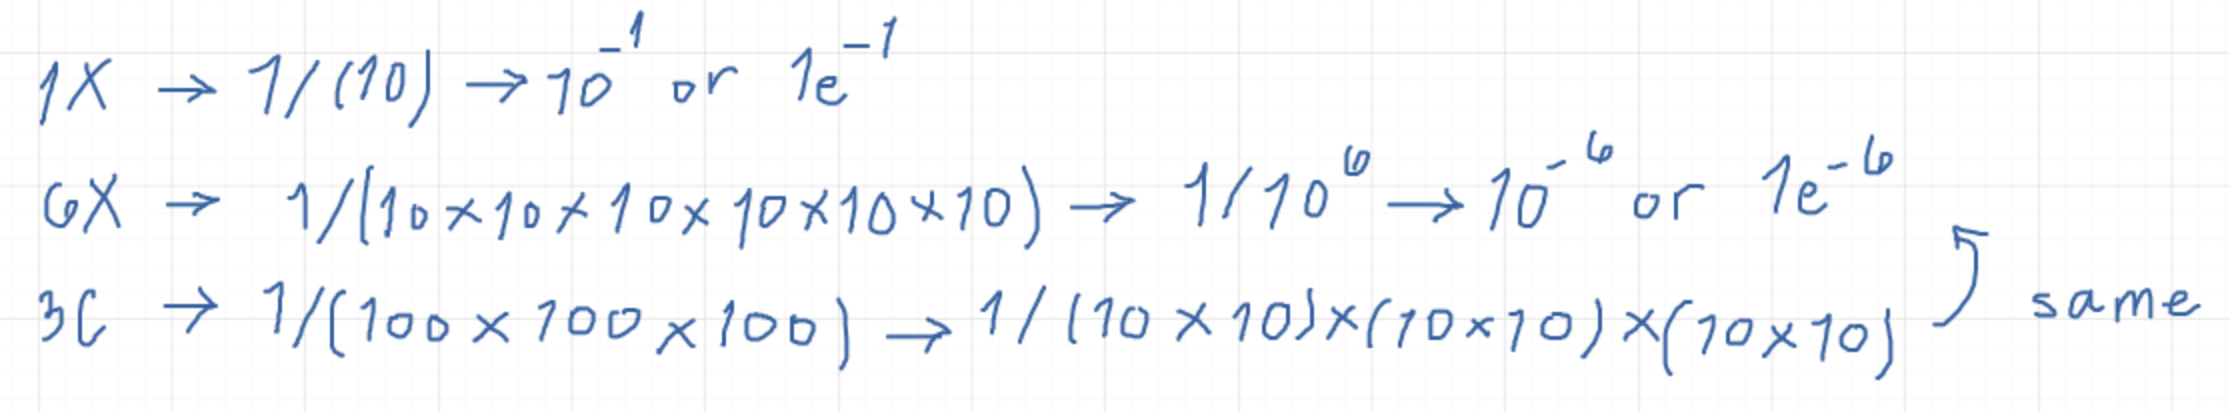
\includegraphics[trim=1cm 1cm 1cm 0cm, width=5in]{units.png}
\end{center}
\end{figure}

\begin{enumerate}
\item A 30C (60X) solution was advocated frequently by Hahnemann. What fraction of the dose will be the active ingredient?

\item The homeopathic flu remedy Oscillococcinum is diluted to 200C. There are $\sim 10^{80}$ atoms in the observable universe. How many observable universes are required to find one molecule of duck liver, the active ingredient?

\item Do you find it plausible that homeopathic remedies outperform placebos?
\ \\
\ \\
\noindent One of our TAs went down to the corner pharmacy (at 120th and Amsterdam) and sure enough, there were plenty of homeopathic remedies nestled between actual medicines. Here are some pictures from her recon:
\begin{figure}[h!]
\begin{center}
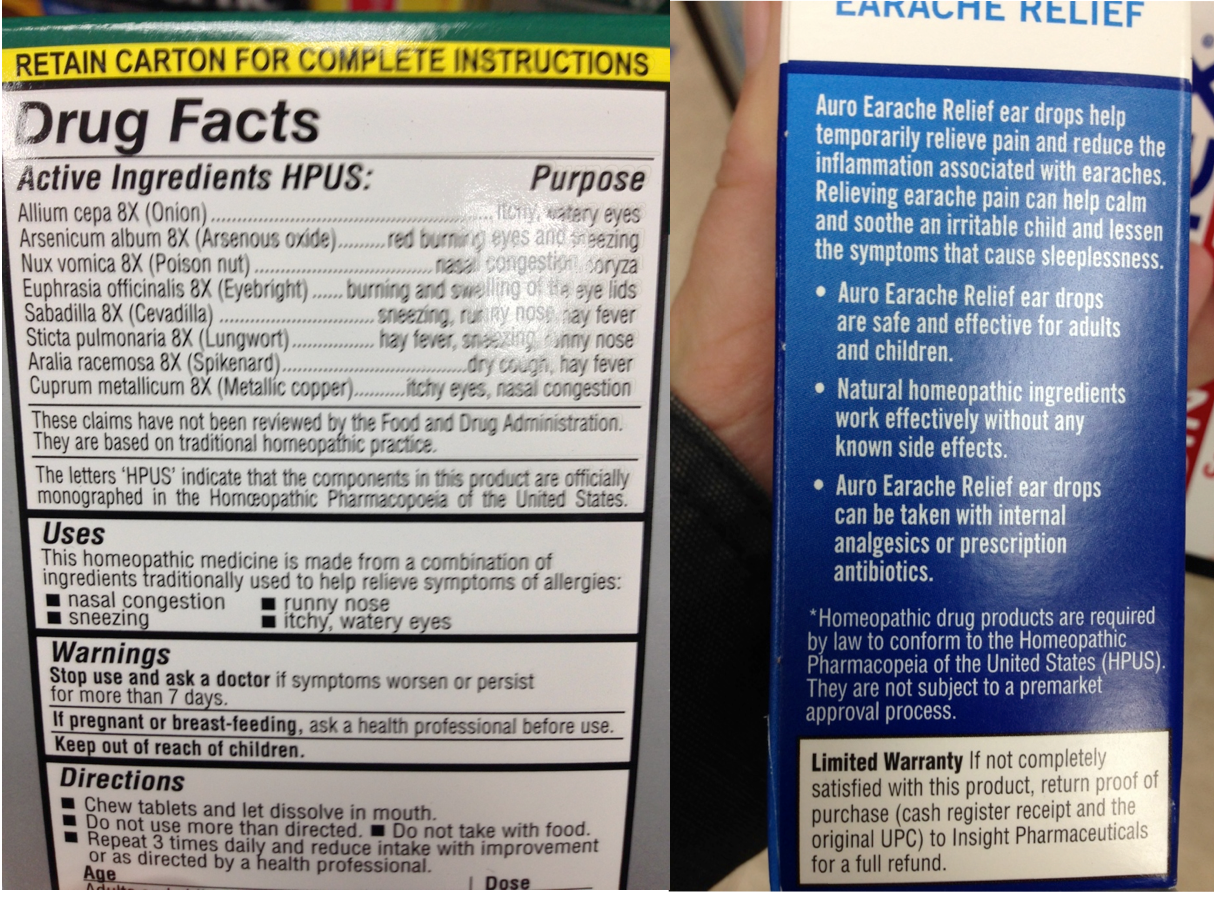
\includegraphics[trim=1cm 1cm 1cm 0cm, width=4.5in]{homeo3.png}
\end{center}
\end{figure}
\noindent The lefthand picture is a homeopathic remedy that is supposed to relieve allergies. As you can see, various ingredients are diluted 8X. 


\item Let's do a fun little comparison. The EPA has set the allowable concentration of arsenic in drinking water at 0.010 parts per million. How does the concentration of arsenic in your water compare to the concentration of onion, poison nut, etc. in this homeopathic remedy (Hint: 0.01 ppm is 1/$10^8$)?
\end{enumerate}

\noindent The second picture is an opportunity to think about public policy related to homeopathy. This is the back of a homeopathic earache remedy. Note the warning ``Homeopathic drug products are required by law to conform to the Homeopathic Pharmacopeia of the United States (HPUS). They are not subject to a premarket approval process." The HPUS is the result of the Federal Food, Drug, \& Cosmetic Act of 1938, which created several loopholes in the normal drug-approval process that allow homeopathic remedies to forgo the normal FDA drug approval process. According to the FDA, ``a product's compliance with the requirements of the HPUS, USP, or NF does not establish that it has been shown by appropriate means to be safe, effective, and not misbranded for its intended use." [Source: CPG Sec. 400.400: Conditions Under Which Homeopathic Drugs May be Marketed, fda.gov]
\begin{itemize}
\item Discuss with a classmate and reflect on the implications of this policy. 
\end{itemize}

\noindent Perhaps not surprisingly, there are many that take issue with the current US policy on homeopathic remedies. In 2011, a class action lawsuit was filed against Boiron, Inc., the company that sells a brand of the homeopathic flu treatment Oscillococcinum (Oscillo) that we examined above. The company was charged with false advertising, making misleading claims, etc. Oscillococcinum does not outperform placebo in scientific trials, and duck liver (the active ingredient) has no scientifically verified medical properties. The case settled out of court, with no admission of wrongdoing from Boiron. Asked whether Oscillo is safe, Boiron spokesperson Gina Casey replied ``Of course it is safe. There's nothing in it." [Sources: US News \& World Report, Top Class Actions]

\begin{itemize}
\item What do you think public policy on homeopathic remedies should be? Is it okay as is, or should it be changed? Why?
\item A 6-pack of Oscillococcinum pills is currently \$14.49 on the Walgreens website. What are the ethical implications of selling a \$14.49 pack of sugar pills? 
\end{itemize}

\section{Conclusion}
For discussion:
\begin{itemize}
\item Given all that we have discussed, why do you think people believe in pseudoscience? Why might it be difficult to dissuade people of their pseudoscientific beliefs?
\item What does Carl Sagan's book chapter have to do with our discussion today?
\end{itemize}
Answer in your notebook:
\begin{enumerate}
\item How can you distinguish between science and pseudoscience in your everyday life? 
\item What are some instances in which you might have to?
\item What is a question or comment you have about today's lab?
\end{enumerate}


\end{document}

